	\documentclass[11pt, letterpaper]{report}
\usepackage{amsmath,fullpage,graphicx,amssymb}

\setlength{\parindent}{0em}

\newcommand{\nott}{{\sim}}

\newcommand{\Z}{\mathbb{Z}}
\newcommand{\R}{\mathbb{R}}

\newcommand{\powerset}[1]{\mathcal P \left({#1}\right)}

\newcommand{\proofnote}[1]{[\textit{Note: #1}]}

\begin{document}

{\textbf{Discrete Structures, Fall 2017, Homework 11 Solutions}}

\vspace*{.1in}

You must write the solutions to these problems legibly on your own paper, with
the problems in sequential order, and with all sheets stapled together.

\bigskip

\begin{enumerate}

\item Let $X = \{1,2,3,4,5\}$ and  $Y=\{a,b,c,d,e\}$.  Define $f:X\to Y$ as follows: $f(1)=a$, $f(2)=b$, 
$f(3)=b$, $f(4)=e$, and $f(5)=d$.
\begin{enumerate}
	\item Draw an arrow diagram for $f$.
	
	\textbf{Solution:}
	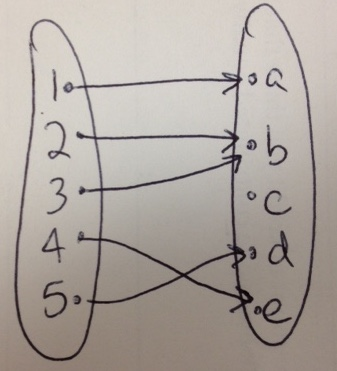
\includegraphics[scale=0.4]{hw10image1.jpg}
	
	\item Let $A= \{1,2,3\}$, $S=\{a\}$, $T=\{b,c,d\}$, and $W=\{c\}$.  Find $f(A)$, $f(X)$, $f^{-1}(S)$, $f^{-1}(T)$, $f^{-1}(W)$, and $f^{-1}(Y)$.  [Remember that images and pre-images/inverse images are sets!]

	
	\textbf{Solution:}
	
	$f(A) = \{a,b\}$
	
	$f(X) = \{a,b,d,e\}$ 
	
	$f^{-1}(S) = \{1\}$
	
	$f^{-1}(T) = \{2,3,5\}$
	
	$f^{-1}(W) = \{\} = \emptyset$  (note, not $\{\emptyset\}$)
	
	$f^{-1}(Y) = \{1,2,3,4,5\} = X$
\end{enumerate}

\item Define $f : \R \to \R$ by the rule $f(x) = x^3-1$.  
\begin{enumerate}
\item Is $f$ 1-1?  Prove or give a counterexample.

\textbf{Solution:}

$f$ is 1-1.  

Proof:

Let $x_1$ and $x_2$ be arbitrary elements in $\R$.  Assume that $f(x_1) = f(x_2)$.

By the definition of $f$, we know $x_1^3-1 = x_2^3-1$.

Add 1 both sides to get $x_1^3 = x_2^3$.

We can take the cube root of each side to get $x_1=x_2$.

\proofnote{We can take the cube root because if $a^3=b^3$, $a$ must equal $b$.  This is
not true for even powers.}

By closing the conditional world and universal generalization, we know  \\
$\forall x_1,x_2 \in \R \ f(x_1) = f(x_2) \to x_1=x_2$.

Therefore, $f$ is 1-1 by the definition of 1-1.


\item Is $f$ onto?  Prove or give a counterexample.

\textbf{Solution:}

$f$ is onto.

Proof:

Let $y$ be an arbitrary element in $\R$.  

Define $x$ to be the real number $\sqrt[3]{y-1}$.

Then $f(x) = f(\sqrt[3]{y-1}) = (\sqrt[3]{y-1})^3 + 1 = (y-1)+1 = y.$

Because we defined an $x$ existentially, we can say $\exists x \in \R \ f(x)=y$.

Because $y$ was chosen arbitrarily, we can say $\forall y \in R \ \exists x \in \R \ f(x)=y$.

Therefore, $f$ is onto by the definition of onto.
\end{enumerate}



\item Let $A = \{1, 2, 3, 4\}$.  Define a function $f:A \to A$ using an arrow diagram such that
$f$ is 1-1 and onto, $f$ \textbf{is not} the identity function, but $f \circ f$ \textbf{is} the identity function.

\textbf{Solution:}

\proofnote{There are lots of solutions to this problem.  Here's one.}

(Imagine the following function as an arrow diagram.)

Choose $f(1) = 2, f(2) = 1, f(3) = 4, f(4) = 3$.  Clearly $f$ is 1-1 and onto, and $f$ is
not the identity function.  However, note that $(f \circ f)(x) = f(f(x)) = x$ for all
$x \in A$, so $f \circ f$ is the identity function.

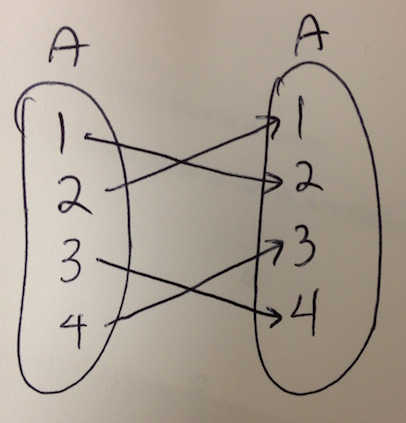
\includegraphics[scale=0.3]{hw10image3.jpg}




\item Let $X$, $Y$, and $Z$ be any sets.  Suppose $f:X\to Y$ and $g: Y \to Z$ are functions.
If $g \circ f$ is 1-1, must it be true that $f$ is 1-1?  Prove or give a counter-example.

\textbf{Solution:}

It is true that $f$ must be 1-1 if you know $g \circ f$ is 1-1.

Proof:

\proofnote{We want to prove that $f$ is 1-1.  We will put the definition of $f$ here
(not in the proof, but off to the side) so we know what we're aiming for:
$\forall x_1, x_2 \in X \ f(x_1) = f(x_2) \to x_1 = x_2$.}

Suppose $x_1$ and $x_2$ are arbitrary elements in $X$.  Assume that $f(x_1) = f(x_2)$.

We know that $g \circ f$ is 1-1, so let's invoke that definition:\\
We know $\forall x_1, x_2 \in X \ (g \circ f)(x_1) = (g \circ f)(x_2) \to x_1 = x_2$.

Apply $g$ to both sides of $f(x_1) = f(x_2)$ to get $g(f(x_1)) = g(f(x_2))$.

Use the definition of function composition to get $(g \circ f)(x_1) = (g \circ f)(x_2)$.

Therefore, by universal modus ponens, we know $x_1=x_2$.  [\textit{We are referencing the earlier fact that $g\circ f$ is 1-1.}]

By closing the conditional world and universal generalization, we know  \\
$\forall x_1, x_2 \in X \ f(x_1) = f(x_2) \to x_1 = x_2$.

Therefore, $f$ is 1-1 by the definition of 1-1.


\item Let $X$, $Y$, and $Z$ be any sets.  Suppose $f:X\to Y$ and $g: Y \to Z$ are functions.
If $g \circ f$ is 1-1, must it be true that $g$ is 1-1?  Prove or give a counter-example.

\textbf{Solution:}

It is \textbf{not} true that $g$ must be 1-1 if you know $g \circ f$ is 1-1.  In other words, it
is possible for $g$ to not be 1-1.

Counterexample:

Define sets $X=\{a,b\}, Y=\{1,2,3,4\}, Z=\{i,j,k\}$. 

 Define $f:X \to Y$ as $f(a)=1$
and $f(b) = 2$.  

Define $g:Y\to Z$ as $g(1)=i$, $g(2)=j$, and $g(3)=g(4)=k$.

Then $g \circ f$ can be computed as $(g \circ f)(a) = g(f(a)) = g(1)=i$, and 
$(g \circ f)(b) = g(f(b)) = g(2)=j$.

Clearly, $g\circ f$ is 1-1, but $g$ is not 1-1.

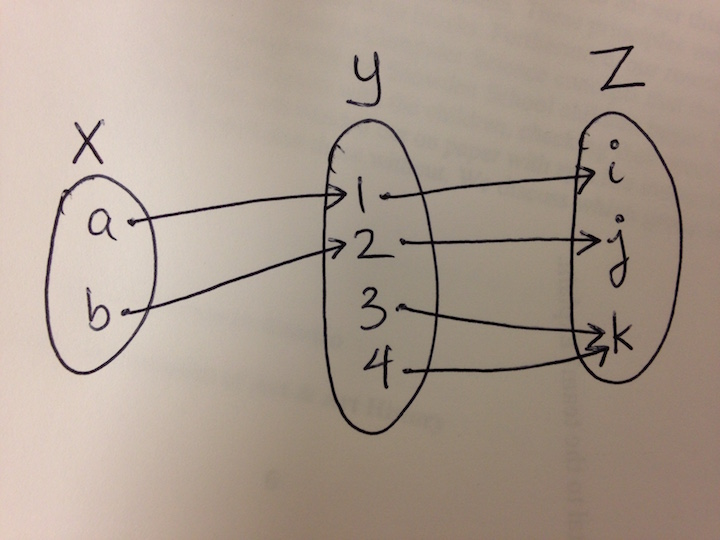
\includegraphics[scale=0.3]{hw10image2.jpg}

\proofnote{The trick in this counterexample is to make sure that the elements of $Y$ that
break the one-to-one-ness of $g$ are not elements that are mapped to by any elements in $X$.}


\end{enumerate}
\bigskip

\end{document}